\documentclass[10pt,letterpaper]{article}
\usepackage[T1]{fontenc}
\usepackage[utf8]{inputenc}
\usepackage{lmodern}
\usepackage[margin=0.88in]{geometry}
\usepackage{microtype}
\usepackage{amsmath,amssymb,mathtools}
\usepackage{graphicx}
\usepackage{booktabs,tabularx,array}
\usepackage{enumitem}
\usepackage[font=small,labelfont=bf]{caption}
\usepackage{float}
\usepackage{hyperref}
\def\UrlBreaks{\do\/\do-\do\_\do\.}
\hypersetup{
  colorlinks=true,
  linkcolor=black,
  citecolor=black,
  urlcolor=blue,
  pdftitle={From Shared Weights to Head-Orthogonal Fibers: Virtual Depth, Head-Readable Staircases, and Post-Stall Search in Looped Transformers},
  pdfauthor={Patrick Dugan}
}
\setlength{\parindent}{1.1em}
\setlength{\parskip}{0.16em}
\setlist[itemize]{topsep=3pt,itemsep=1.5pt,leftmargin=*}
\renewcommand{\arraystretch}{1.12}

\newcommand{\LoopT}{\textsc{Loop-T}}
\newcommand{\FFU}{\textsc{FF-U}}
\newcommand{\EM}{\ensuremath{\mathrm{EM}}}
\newcommand{\IIA}{\ensuremath{\mathrm{IIA}}}
\newcommand{\DEF}{\ensuremath{\mathrm{DEF}}}
\newcommand{\cur}{\operatorname{cur\_node}}
\newcommand{\Gprop}{G_{\mathrm{prop}}}
\newcommand{\Phead}{P_{\mathrm{head}}}

\title{\bfseries From Shared Weights to Head-Orthogonal Fibers:\\[0.30em]
Virtual Depth, Head-Readable Staircases, and\\[0.14em]
Post-Stall Search in Looped Transformers}
\author{Patrick Dugan}
\date{November 2026\\[0.2em]\normalsize Unified synthesis across six studies: \texttt{VPD}, \texttt{HUG-CAL-02}, \texttt{RMP}, \texttt{LOOPSCOPE-01}, \texttt{ARG-02}, and \texttt{LOOPSCOPE-02}}

\begin{document}
\maketitle
\vspace{-0.70em}

\begin{abstract}
\noindent
Weight-tied transformers reuse identical parameters across sequential passes, yet parameter sharing spans distinct computational regimes whose capability gains, failure modes, and latent-state monitorability differ sharply. Synthesizing six studies across four experimental arcs—pretrained looped language models (\texttt{Nanbeige4.2-3B}, \texttt{Huginn-0125}), controlled algorithmic loopers (\LoopT, \texttt{LoopedChase}, \texttt{Lean-CGRT}), untied baselines (\FFU, \texttt{Qwen3.5-4B-Base}, \texttt{Qwen3-4B-Instruct}), and 7M-parameter convergent Tiny Recursive Models (\texttt{TRM})—we separate weight sharing into three mechanistic regimes. First, two-pass language models implement \emph{fixed-pass virtual depth}: \texttt{Nanbeige4.2-3B} routes SwiGLU inputs through layer-selectively distinct singular subspaces across passes (mean top-64 SVD usage correlation $\bar{r}=0.355$; $r=0.085$ at \texttt{L12.mlp.down\_proj}) and rotates downstream perturbation directions when loop-boundary state is carried rather than reset, while discrete Top-32 sparse autoencoder support switches limit intervention-change fidelity ($F_\Delta > 0$ in $1/12$ second-pass \texttt{L22} edits despite Muon lifting state explained variance from $-0.180$ to $+0.453$). Across pointer chasing, 168-case finite-group composition (\texttt{ARG-02}: $65/168 = 38.7\%$ at native $t=2$, $76/168 = 45.2\%$ at $t=4$ [$p=0.080$], $71/168 = 42.3\%$ at $d^*=8$ [$p=0.61$]), and deductively stratified $9\times 9$ Sudoku (\texttt{LOOPSCOPE-02}), \texttt{Nanbeige4.2-3B} fails its registered recurrent gate (\texttt{H2a} $p=0.097$) and trails untied \texttt{Qwen3.5-4B-Base} on immediate single-cell elimination (\texttt{S1}: $11/64$ vs.\ $30/64$; overall $0.129$ vs.\ $0.211$, $p=0.0031$) while both sit near the $1/9 \approx 0.111$ uniform floor on multi-step strata (\texttt{S2--S4}). Second, multi-iteration BPTT loopers exhibit \emph{dynamical settling and head-readable staircases}: activation-matched input rotations on \texttt{Huginn-0125} (\texttt{HUG-CAL-02}) eliminate apparent late-iteration SVD specialization ($\pm 0.0065$ nats), motivating \emph{Transported Component Attribution} (\texttt{TCA}), which separates dynamical fragility from closed-form directional specificity in one backward pass ($\rho=0.75$ across 480 \texttt{Huginn} conditions) and exposes an observational Lyapunov contrast between BPTT and 1-step detached ACT ($F_1/F_6 = 1{,}808.4$ across 126 core calls despite $0.303\times$ finite kick contraction, alongside $22.04\%$ read-specific components). On Markovian pointer chains, $\lambda \ge 0.1$ achieves $1.00$ depth-9--16 extrapolation and $1.00$ head readability, own-head commutation predicts extrapolation at $\mathrm{AUC}=0.992$, and projecting the carried cursor onto the 16-d readout row space ($\Phead$) at $\lambda=0.1$ retains $1.000$ extrapolation. Third, on $9\times 9$ Sudoku, a 7M \texttt{TRM} (16 outer steps $\times$ 21 core calls $= 336$ passes) solves $88.3\%$ ($226/256$) of \texttt{items256} and $100\%$ ($100/100$) of \texttt{bench100} ($92/100 = 92.0\%$ on an independent replication checkpoint), including $51/51$ (\texttt{bench100}) and $153/183 = 83.6\%$ (\texttt{items256}) whole-board deductively stalled puzzles. Visible beliefs commute with exact propagation before stall ($\mathrm{AUC}=1.000$). While naive unnormalized projection onto the 11-d \texttt{lm\_head} row space collapses solve ($1.000 \to 0.050$--$0.070$) via off-manifold norm loss, restoring per-cell L2 norm, train-mean offset, or donor fibers preserves $100\%$ ($73/73$) of propagation-solvable boards and $74.9\%$--$76.0\%$ of stalled \texttt{items256} boards via continuous $81\times 11$ logit fields, isolating a selective $-7.7$ to $-8.7$~pp deficit on stalled boards ($p \le 0.0043$; $-15.6$~pp on round-0 stalled \texttt{S4}, $-21.9$~pp under step-1 fiber freeze, $p=1.08\times 10^{-6}$) that recovers completely with the top $k=64$ orthogonal PCA directions ($p=1.00$) and remains linearly probe-decodable ($97.1\%$--$97.8\%$ step-1 candidate masks; $93.5\%$--$100\%$ step-16 digits).
\end{abstract}

\section{Introduction: Three Regimes of Weight Sharing}\label{sec:intro}

A weight-tied transformer applies identical block parameters $\theta$ across $T$ sequential passes \cite{dehghani2019universal,giannou2023looped,saunshi2025latent,geiping2025huginn,wang2025hrm,jolicoeur2025trm,li2026deeploop}. Because parameter identity no longer indexes computational depth, two questions govern capability and interpretability in recurrent-depth architectures:
\begin{enumerate}[topsep=3pt,itemsep=2pt]
  \item \textbf{Capability triangulation:} When does reusing $\theta$ across passes yield multi-step algorithmic or combinatorial reasoning beyond an untied transformer, and what dynamical invariants separate fixed-pass stage pipelines from convergent recursive solvers?
  \item \textbf{Latent monitorability:} When can intermediate computation be audited directly through the output readout head $\Phead$, when does state orthogonal to the readout ($\ker(\texttt{lm\_head})$) carry causal search information, and is that head-orthogonal state opaque to linear probes or merely invisible to token logits?
\end{enumerate}

Our September 2026 study of the pretrained two-pass language model \texttt{Nanbeige4.2-3B} \cite{nanbeige2026model,dugan2026vpd} examined shared MLP matrices via multipass vector parameter decomposition (\texttt{VPD}) \cite{braun2025apd} and shared Top-32 sparse autoencoders (\texttt{SAE}s) \cite{bricken2023monosemanticity,gao2024scaling} across \texttt{ARC-AGI-1}, \texttt{ARC-AGI-2}, and Prime Intellect's \texttt{INTELLECT-3} public reinforcement-learning logic and mathematics reasoning corpus \cite{primeintellect2025intellect3}. That study found sharp terminal-layer pass divergence, showed that Muon-hybrid optimization \cite{jordan2024muon,dugan2026muonsae} rescues second-pass state reconstruction without rescuing intervention-change fidelity, and proved via a 44-layer embedding-reset control that carrying loop-boundary state rotates downstream perturbation directions. Yet it left open whether two-pass reuse buys multi-step deduction, whether per-iteration weight-ablation asymmetries reflect specialized factors or dynamical sensitivity, and where the boundary lies between head-readable iteration and head-orthogonal state.

Over the subsequent ten weeks, five concurrent looped-transformer interpretability papers established key properties of recurrent computation while leaving these questions open (Table~\ref{tab:literature}). Blayney et al.\ \cite{blayney2026mechanistic} analyzed cyclic fixed points and the stabilizing roles of input injection and normalization; Kaissis et al.\ \cite{kaissis2026sdi} introduced Step-Decomposed Influence (\texttt{SDI}) to decompose TracIn training-data influence across BPTT iterations via gradient--activation outer products; Wu, Hu, and Zhang \cite{wu2026shared} introduced \texttt{J}-steering—learning a linear map $J$ on the incoming hidden state of a frozen loop—and observed that loop predictions advance by uneven per-step distances or stall; Sesodia et al.\ \cite{sesodia2026inside} demonstrated that weight-tied transformers outperform identically trained untied models of equal effective depth on depth-bound tasks while forming iteration-budget staircases; and Olszowiec et al.\ \cite{olszowiec2026monitoring} compared eight looped language models, showing that hidden-state stability and latent reasoning depend strongly on whether input embeddings are re-injected at each loop iteration.

\begin{table}[t]
\centering
\small
\begin{tabularx}{\linewidth}{@{}l>{\raggedright\arraybackslash}p{0.33\linewidth}>{\raggedright\arraybackslash}X@{}}
\toprule
Concurrent study & Principal contribution & Complementary contribution in this synthesis \\
\midrule
Blayney et al.\ \cite{blayney2026mechanistic} & Cyclic fixed points and normalization / injection effects in looped LMs & Contrasts non-contractive 2-pass LMs (\texttt{Nanbeige-3B}) against basin-contractive 336-call \texttt{TRM}s on identical Sudoku strata \\
Kaissis et al.\ (\texttt{SDI}) \cite{kaissis2026sdi} & Decomposes TracIn data influence across BPTT loops via $\sum \delta_s \otimes a_s$ & Analytical caution: detached-ACT tangent Jacobians inflate step-1 norms by $1{,}808\times$ ($6{,}400\times$ max); \texttt{TCA} cancels $\|A_s\|$ via rotation nulls \\
Wu, Hu \& Zhang \cite{wu2026shared} & Learned linear \texttt{J}-steering of frozen loops; uneven per-step logit progress & Quantifies cross-pass SVD input multiplexing ($\bar{r}=0.355$) vs.\ stationary \texttt{TRM} reuse ($\bar{r}=0.992$) and 48-cycle lock-in staircases \\
Sesodia et al.\ \cite{sesodia2026inside} & Weight-tied beats matched untied training; iteration-budget staircases & Replicates matched-training advantage in \LoopT\ vs.\ \FFU; shows $\Gprop$ belief commutation ($\mathrm{AUC}=1.000$) before deductive stall \\
Olszowiec et al.\ \cite{olszowiec2026monitoring} & Prompt re-injection governs trajectory stability across 8 looped LMs & Audits input re-injection across all 6 model families and isolates on-manifold $\Phead$ vs.\ head-orthogonal search residuals \\
\bottomrule
\end{tabularx}
\caption{Positioning relative to concurrent 2026 looped-transformer interpretability studies.}
\label{tab:literature}
\end{table}

Synthesizing six studies across four experimental arcs—September \texttt{VPD} \cite{dugan2026vpd}, registered \texttt{Huginn-0125} calibration (\path{HUG-CAL-02} \cite{dugan2026hugcal}), controlled closed-loop mediation and compactification (\texttt{RMP} \cite{dugan2026rmp}, \path{LOOPSCOPE-01} \cite{dugan2026loopscope01}, \path{ARG-02} \cite{dugan2026arg02}), and stratified $9\times 9$ Sudoku triangulation with head-orthogonal manifold controls (\path{LOOPSCOPE-02})—we establish three mechanistic regimes:
\begin{itemize}
  \item \textbf{Regime I — Fixed-Pass Virtual Depth (Section~\ref{sec:regime1}):} Without input re-injection, fixed $T=2$ \texttt{Nanbeige4.2-3B} routes nonlinear MLP activations through pass-divergent singular subspaces ($\bar{r}=0.355$) as a compressed 44-layer pipeline, failing to contract perturbations ($6.9\times$ amplification) or clear multi-step deductive strata.
  \item \textbf{Regime II — Dynamical Settling and Head-Readable Staircases (Sections~\ref{sec:fragility}--\ref{sec:regime2}):} In multi-step BPTT loopers, apparent late-loop SVD specialization on \texttt{Huginn-0125} vanishes under activation-matched input rotations (\texttt{HUG-CAL-02}), formalized in one pass by \texttt{TCA}. On Markovian chains (\texttt{LoopedChase}), per-loop supervision ($\lambda=0.1$) yields $1.000$ OOD extrapolation, $\mathrm{AUC}=0.992$ belief commutation, and $1.000$ retention when 240 of 256 cursor dimensions orthogonal to $\Phead$ are erased every loop.
  \item \textbf{Regime III — Stationary Attractor Search and Head-Orthogonal Residual Memory (Section~\ref{sec:regime3}):} A 7M Sudoku \texttt{TRM} (336 core calls with input re-injection) iterates a stationary outer operator ($\bar{r}_{\mathrm{outer}}=0.992$) that contracts finite kicks ($0.303\times$) and repairs 10-cell corruptions ($0.000 \to 0.887$). Controlling for off-manifold L2 norm loss—which confounded unnormalized $\Phead$ erasure—proves that $100\%$ of propagation-solvable boards and $\approx 75\%$ of stalled boards solve via the continuous $81\times 11$ head-space logit field alone, while a linearly decodable, top-64 PCA subspace inside the 501-d head-orthogonal complement $\ker(\texttt{lm\_head})$ supplies the remaining $+7.7$ to $+8.7$~pp on stalled boards ($+15.6$~pp on round-0 stalled \texttt{S4}).
\end{itemize}

\paragraph{Provenance and archival discipline.} Pre-registered decision rules and post-hoc controls are kept strictly distinct: all composite verdicts that returned \texttt{Not supported} or \texttt{Weak} (\texttt{HUG-CAL-02}, \texttt{ARG-02} \texttt{H2a}, and \texttt{LOOPSCOPE-02} \texttt{P1}--\texttt{P4}) are reported verbatim alongside their sub-metrics, and our post-hoc manifold/PCA controls on \texttt{P5} explicitly correct an unnormalized projection confound in archival snapshot \texttt{v009} while leaving \texttt{VPD} \texttt{v001}--\texttt{v010} and \texttt{papers/rmp\_looped\_mechinterp} unmodified.

\section{Regime I: Two-Pass Virtual Depth, Support Switching, and SVD Multiplexing}\label{sec:regime1}

We first examine \texttt{Nanbeige/Nanbeige4.2-3B} \cite{nanbeige2026model} (revision \texttt{451ed48c}), a pretrained decoder executing 22 shared transformer layers twice per forward pass ($T=2$, 44 executed layers) with a loop-boundary \texttt{RMSNorm} and \emph{no} re-injection of token embeddings before Pass 2.

\subsection{Terminal Pass Divergence and the Muon SAE Fidelity Gap}

In \cite{dugan2026vpd}, a 64-component multipass \texttt{VPD} decomposition (\texttt{prime-20260906T204058Z-561}, capturing $\approx 2.2\%$ of squared weight norm at \texttt{mlp.down\_proj} of physical layers 12 and 22) and shared 6,144-latent Top-32 \texttt{SAE}s were evaluated on 18 reasoning trajectories (8 calibration, 10 held-out across 8 task groups) from \texttt{ARC-AGI-1}, \texttt{ARC-AGI-2}, and \texttt{INTELLECT-3} logic and mathematics \cite{primeintellect2025intellect3}. Residual-stream cosine similarity between Pass 1 and Pass 2 stays high at physical mid-layer \texttt{L12} ($0.799$--$0.869$) but drops sharply at terminal physical layer \texttt{L22} to $0.230$--$0.307$ ($0.184$--$0.229$ post-loop-norm), already within the prompt suffix before generation.

Fitting one shared Top-32 \texttt{SAE} across both passes under AdamW yielded negative held-out \texttt{L22} Pass-2 state explained variance ($\mathrm{EV} = -0.180$ on Q4 trajectories; $-0.535$ on BF16 intervention baselines, vs.\ $+0.830$ and $+0.763$ on Pass 1). Switching matrix parameters to Muon \cite{jordan2024muon,dugan2026muonsae} rescued static reconstruction ($\mathrm{EV} = +0.453$ Q4, $+0.312$ BF16 on Pass 2; $0.918$ and $0.942$ on Pass 1), yet failed to rescue \emph{intervention-change fidelity} for true shift $\Delta h = h_1 - h_0$ and reconstructed shift $\Delta \hat{h} = \hat{h}_1 - \hat{h}_0$ ($e(h)=h-\hat{h}$):
\begin{equation}
  F_\Delta \;=\; 1 - \frac{\|\Delta h - \Delta \hat{h}\|_2^2}{\|\Delta h\|_2^2}
  \;=\; 1 - \frac{\|e(h_1) - e(h_0)\|_2^2}{\|\Delta h\|_2^2}.
  \label{eq:fdelta}
\end{equation}
Muon improved \texttt{L22} Pass-2 $F_\Delta$ in $12/12$ conditions ($18/20$ nonzero \texttt{L22} conditions overall), but only $1/12$ exceeded zero ($+0.030$). Discrete Top-32 encoder support switches at $1$--$3$ of $80$ positions caused $93.3\%$--$99.6\%$ of change-mismatch energy; freezing baseline active support reduced a unit-write mismatch from $-52.367$ to $-0.000543$. A 44-layer \emph{embedding-reset control} replacing Pass-1 output with token embeddings matched 22-layer one-pass states bit-for-bit across 150 pairs and kept propagated \texttt{L12}$\to$\texttt{L22} Muon $F_\Delta$ positive ($+0.047$ to $+0.572$) versus negative under state carry ($-0.300$ to $-0.046$); crossing baselines with unit response directions confirmed that state carry rotates downstream Jacobian directions ($0.059/0.051$ carry vs.\ $0.354/0.377$ reset).

\subsection{Triangulating Pretrained Capability Across Pointer Chasing, Algebra, and Sudoku}

Unlike matched-training studies where weight-tied models outperform depth-matched untied baselines trained on the same corpus \cite{sesodia2026inside} (replicated in our controlled \LoopT\ vs.\ \FFU\ experiments in Section~\ref{sec:regime2}), comparing pretrained \texttt{Nanbeige4.2-3B} against untied \texttt{Qwen} checkpoints is observational across model families, parameter counts, and pretraining mixtures; it tests whether \texttt{Nanbeige}'s two-pass reuse exhibits iterative scaling at inference (Figure~\ref{fig:triangulation}, Table~\ref{tab:sudoku_triangulation}):
\begin{enumerate}[topsep=3pt,itemsep=2pt]
  \item \textbf{Pointer chasing (\texttt{Silico Stage 1}):} On 3-shot 16-node chains, \texttt{Nanbeige4.2-3B} scores $79.2\%$ at 1 hop (chance $6.25\%$) and $6.55\%$ ($131/2{,}000$) across depths 3--6, with Pass-1-only sensitivity on top \texttt{L22} \texttt{VPD} factors \texttt{(19, 9, 43)} ($-0.060$ to $-0.098$ nats on Pass 1; $0.000$ on Pass 2).
  \item \textbf{Finite-group composition (\texttt{ARG-02} Extension N1 \cite{dugan2026arg02}):} On $N=168$ held-out group trace items (\texttt{future@12}, dev-selected budget $d^*=8$ from 132 dev items), \texttt{Nanbeige4.2-3B} solves $44/168$ ($26.2\%$) at $t=1$, $65/168$ ($38.7\%$) at native $t=2$ ($+21$ items, McNemar $p=0.040$), $76/168$ ($45.2\%$) at OOD $t=4$ ($+11$ over $t=2$, $p=0.080$), and $71/168$ ($42.3\%$) at $d^*=8$ ($+6$ over $t=2$, $p=0.61$), compared with single-pass \texttt{Qwen3.5-0.8B} ($68/168 = 40.5\%$) and \texttt{Qwen3.5-2B} ($79/168 = 47.0\%$). Thus OOD loops $t=4,8$ show positive point-estimate gains over $t=2$ that do not reach statistical significance. Pre-registered recurrent mechanism gate \texttt{H2a}—requiring closed-loop $d^*=8$ ($71/168$) to significantly beat linear open-loop extrapolation $h_{\mathrm{open}}(t) = h(1) + (t-1)(h(1)-x)$ ($55/168 = 32.7\%$ at both $t=2$ and $t=8$)—failed ($+16$ items, $p=0.097$); donor-shuffled Pass-2 displacements scored $69/168$ ($41.1\%$, differing from clean $t=2$ on $6/168$ items), and $0.25\cdot\mathrm{RMS}$ kicks amplified by $2.8\times \to 3.9\times \to 6.9\times$ across loops $2, 4, 8$.
  \item \textbf{Stratified $9\times 9$ Sudoku (\texttt{LOOPSCOPE-02}):} Across 256 held-out \texttt{sudoku-extreme} boards stratified into $n=64$ per deductive round class of exact synchronous naked- plus hidden-single propagation $\Gprop$—\texttt{S1\_naked1} ($r=1$), \texttt{S2\_prop2} ($r=2$), \texttt{S3\_prop3plus} ($r\ge 3$), and \texttt{S4\_stalled} (zero singles anywhere on the board at round 0)—single-target-cell 3-shot accuracy is $25/256$ ($0.098$) at $t=1$, $33/256$ ($0.129$) at $t=2$ ($p=0.341$), and $23/256$ ($0.090$) at $t=8$ ($p=0.220$). Crucially, uniform digit guessing gives $1/9 \approx 0.111$ ($\pm 0.077$ two-SE sampling band at $n=64$): every \texttt{Nanbeige} stratum and the \texttt{S2--S4} strata of both \texttt{Qwen} models lie within sampling noise of this floor, so absence of loop scaling cannot be inferred from \texttt{S2--S4} alone. Instead, the entire advantage of untied \texttt{Qwen3.5-4B-Base} ($54/256 = 0.211$, McNemar $p=0.0031$) and pure-SDPA \texttt{Qwen3-4B-Instruct} ($65/256 = 0.254$) over \texttt{Nanbeige} ($t=2$) resides in immediate 1-round elimination \texttt{S1\_naked1} ($30/64 = 0.469$ and $36/64 = 0.562$ vs.\ $11/64 = 0.172$; on \texttt{S2--S4} combined, $24/192 = 0.125$ vs.\ $22/192 = 0.115$, $p=0.824$).
\end{enumerate}

\begin{figure}[t]
\centering
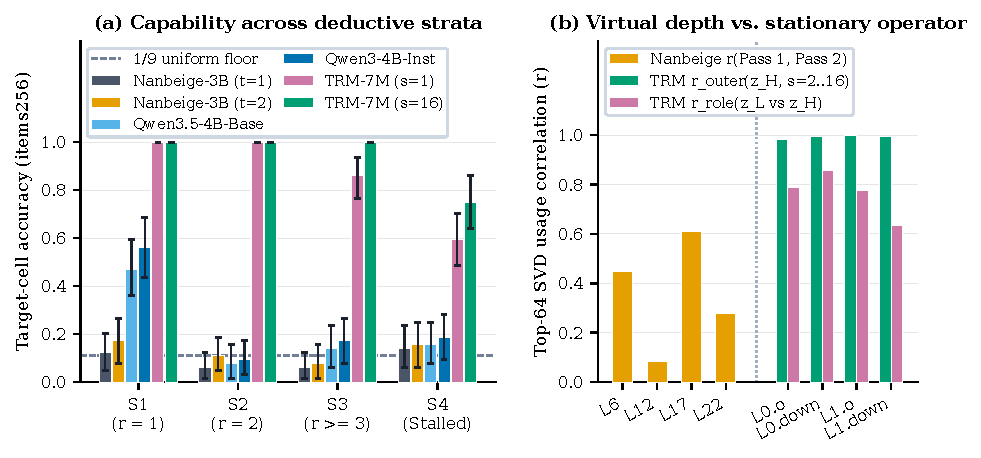
\includegraphics[width=\linewidth]{figures/fig1_virtual_depth_triangulation.pdf}
\caption{\textbf{Regime I vs.\ Regime III on deductively stratified $9\times 9$ Sudoku (\texttt{LOOPSCOPE-02}).} \textbf{(a)} Target-cell accuracy on \texttt{items256} ($n=64$/stratum; 2,000-resample bootstrap 95\% CIs). \texttt{Qwen} models beat \texttt{Nanbeige} strictly on \texttt{S1} ($r=1$), while all three 3B--4B LMs sit near the $1/9 \approx 0.111$ floor on \texttt{S2--S4}; the 7M \texttt{TRM} reaches $1.000$ on \texttt{S1--S3} and $0.750$ target-cell ($0.547$ exact board) on round-0 stalled \texttt{S4}. \textbf{(b)} Top-64 SVD input-usage correlations $r$: \texttt{Nanbeige} multiplexes nonlinear MLP inputs across passes ($\bar{r}=0.355$, $r=0.085$ at \texttt{L12}), whereas \texttt{TRM} iterates a stationary outer operator ($\bar{r}_{\mathrm{outer}}=0.992$) while splitting inner $z_L$ vs.\ $z_H$ calls ($\bar{r}_{\mathrm{role}}=0.765$).}
\label{fig:triangulation}
\end{figure}

\begin{table}[t]
\centering
\small
\begin{tabularx}{\linewidth}{@{}lcccccc>{\raggedright\arraybackslash}X@{}}
\toprule
Model / Pass setting & Params & Overall & \texttt{S1} ($r{=}1$) & \texttt{S2} ($r{=}2$) & \texttt{S3} ($r{\ge}3$) & \texttt{S4} (Stall) & Loop / operator signature \\
\midrule
\texttt{Nanbeige4.2-3B} ($t=1$) & 3.0B & 0.098 & 0.125 & 0.062 & 0.062 & 0.141 & Half virtual pipeline (22L) \\
\texttt{Nanbeige4.2-3B} ($t=2$, native) & 3.0B & 0.129 & 0.172 & 0.109 & 0.078 & 0.156 & Multiplexed SVD ($\bar{r}=0.355$) \\
\texttt{Nanbeige4.2-3B} ($t=8$, OOD) & 3.0B & 0.090 & 0.047 & 0.156 & 0.062 & 0.094 & Non-contractive ($\|\Delta h\|/\|h\|=0.71$) \\
\texttt{Qwen3.5-4B-Base} (untied) & 4.0B & 0.211 & 0.469 & 0.078 & 0.141 & 0.156 & Advantage strictly on \texttt{S1} ($30/64$) \\
\texttt{Qwen3-4B-Instruct} (SDPA) & 4.0B & 0.254 & 0.562 & 0.094 & 0.172 & 0.188 & Untied 36L pure-SDPA control \\
\midrule
\texttt{TRM-7M} ($s=1$: 21 core calls) & 7.0M & 0.863 & 1.000 & 1.000 & 0.859 & 0.594 & Inner sweep; exact board $= 0.082$ \\
\texttt{TRM-7M} ($s=16$: 336 core calls) & 7.0M & \textbf{0.938} & \textbf{1.000} & \textbf{1.000} & \textbf{1.000} & \textbf{0.750} & Stationary ($\bar{r}=0.992$); board $= \mathbf{0.883}$ \\
\bottomrule
\end{tabularx}
\caption{Stratified $9\times 9$ Sudoku target-cell accuracy on \texttt{items256} ($N=256$, $64$ boards/stratum; uniform chance $= 1/9 \approx 0.111$). Note that \texttt{S4} here denotes boards with \emph{zero singles anywhere at round 0} ($n=64$, where \texttt{TRM} $s=16$ target-cell accuracy is $48/64 = 0.750$ and exact 81-cell board solve is $35/64 = 0.547$), distinct from the broader set of $183$ \texttt{items256} boards where whole-board propagation eventually stalls ($153/183 = 0.836$ exact board solve; Table~\ref{tab:fiber_controls}).}
\label{tab:sudoku_triangulation}
\end{table}

\subsection{SVD Input-Subspace Multiplexing and Reconciling \texttt{L12} Residual Alignment}\label{sec:svd_multiplex}

To quantify whether shared matrices execute the same linear sub-operations across passes, let $W_l = \sum_{j} \sigma_{l,j} u_{l,j} v_{l,j}^\top$ be the exact SVD of a shared projection matrix (\texttt{mlp.down\_proj} in \texttt{Nanbeige}; \texttt{o\_proj} and \texttt{down\_proj} in \texttt{TRM}), and define the invocation-$p$ rank-one input-usage profile over top $K=64$ singular directions:
\begin{equation}
  u_{l,p}(j) \;=\; \sigma_{l,j}\,\mathbb{E}_{x \in \mathcal{D}}\bigl[\,|\langle x_{l,p},\, v_{l,j}\rangle|\,\bigr],
  \qquad
  r_l(p,q) \;=\; \operatorname{corr}_{j=1\dots 64}\!\bigl(u_{l,p}(j),\, u_{l,q}(j)\bigr),
  \label{eq:svd_r}
\end{equation}
with $\bar{r}$ denoting the arithmetic mean of $r_l(p,q)$ across audited matrices $l$ (and across outer step pairs $2\le p < q \le 16$ for $\bar{r}_{\mathrm{outer}}$). Across \texttt{Nanbeige} physical layers \texttt{(L6, L12, L17, L22)}, cross-pass correlation averages $\bar{r} = 0.355$ ($r_{\texttt{L6}}=0.448$, $r_{\texttt{L12}}=0.085$, $r_{\texttt{L17}}=0.610$, $r_{\texttt{L22}}=0.277$; Figure~\ref{fig:triangulation}b).

At first glance, near-zero SVD input correlation at \texttt{L12} ($r=0.085$) appears to conflict with high \texttt{L12} residual-stream cosine similarity ($0.799$--$0.869$). The two measurements probe different sites around a nonlinear gate: residual state $h_{12}^{(p)} = h_0^{(p)} + \sum_{\ell \le 12}\Delta_\ell^{(p)}$ is dominated by the shared skip-connection sum accumulated over earlier layers, whereas $x_{\texttt{L12},p}$ entering \texttt{mlp.down\_proj} is the post-\texttt{RMSNorm} \emph{SwiGLU intermediate activation} $\operatorname{SiLU}(W_{\mathrm{gate}}\tilde{h}_{12}^{(p)}) \odot (W_{\mathrm{up}}\tilde{h}_{12}^{(p)})$ in $\mathbb{R}^{d_{\mathrm{ff}}}$. Moderate pass differences in $\tilde{h}_{12}^{(p)}$ switch which multiplicative SwiGLU gates open, routing Pass 1 and Pass 2 into nearly uncorrelated singular input subspaces of \texttt{mlp.down\_proj} even while the ambient residual stream remains macroscopically aligned.

\section{Separating Dynamical Fragility from Component Specificity}\label{sec:fragility}

\subsection{The \texttt{HUG-CAL-02} Rotation Null on \texttt{Huginn-0125}}

On 3-shot variable-binding chains, the 3.5B looped model \texttt{Huginn-0125} \cite{geiping2025huginn} (2-layer prelude, 4-layer tied core unrolled $r=16$ times with learned adapter input re-injection at every step, 2-layer coda) achieves $0.76$ accuracy at 1 hop and $0.47$ at 2 hops ($0.25$--$0.33$ floor at $3$--$6$ hops). Deleting top-16 SVD triplets of core \texttt{mlp.proj} in iterations $1$--$8$ cost $0.00$ nats versus $-0.77$ nats in iterations $13$--$16$. Yet in registered \textbf{Silico Experiment \#3} (\texttt{HUG-CAL-02} \cite{dugan2026hugcal}; 240 clean-correct 2-hop programs $\times$ 3 noise seeds, 8 frozen factors across \texttt{core0--core3}, 4 random orthogonal input-read rotations per factor matched to exact per-iteration projection RMS while fixing write vector $u$), \textbf{factor specialization disappeared}: \texttt{core3 f1} in iterations $9$--$16$ cost $-0.366$ nats raw versus $-0.368$ nats under matched rotation ($+0.0007$ nats net; all 8 factors within $\pm 0.0065$ nats; Figure~\ref{fig:fragility}a). Early ablations are masked by downstream attractor repair; late ablations leave no repair steps before readout.

\begin{figure}[t]
\centering
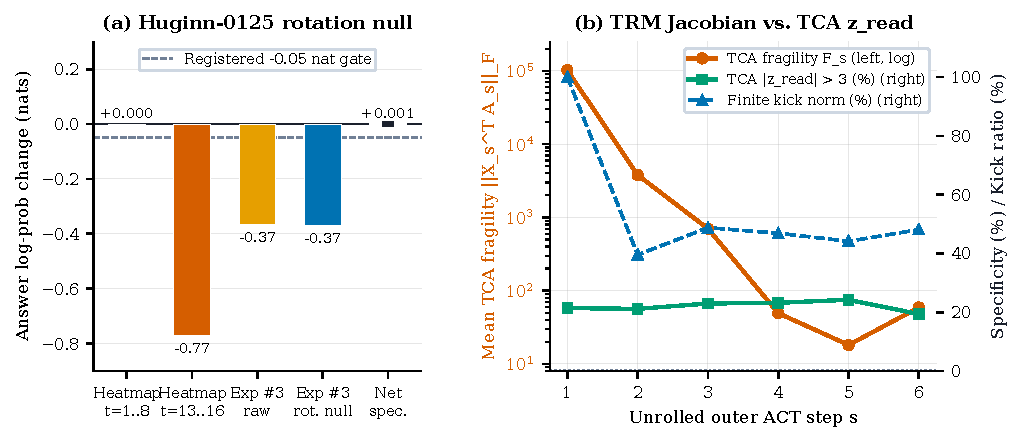
\includegraphics[width=\linewidth]{figures/fig2_fragility_vs_specificity_tca.pdf}
\caption{\textbf{Dynamical fragility vs.\ directional specificity.} \textbf{(a)} Registered \texttt{HUG-CAL-02} (\texttt{Huginn-0125}, $r=16$): late-window SVD ablation loss ($-0.366$ nats) is matched within $\pm 0.0065$ nats by RMS-matched orthogonal read rotations ($-0.368$ nats). \textbf{(b)} Unrolled 6-step \texttt{TCA} on Sudoku \texttt{TRM} (126 core calls; 105 calls between $s=1$ and $s=6$ commits): detached-ACT tangent Jacobians inflate $F_1/F_6 = 1{,}808.4$ while finite $0.25\cdot\mathrm{RMS}$ kicks contract to $30.3\%$; \texttt{TCA}'s rotation $z$-score cancels $\|A_s\|$, isolating a flat $22.04\%$ read-specific circuit.}
\label{fig:fragility}
\end{figure}

\subsection{Transported Component Attribution (\texttt{TCA}) and the Detached-ACT Lyapunov Contrast}

To avoid running multi-pass empirical rotation sweeps per factor, \textbf{Transported Component Attribution (\texttt{TCA})} (\texttt{LOOPSCOPE-01} \cite{dugan2026loopscope01}) computes both fragility and exact Haar-rotation specificity in \emph{one forward and backward pass}. For input activations $X_{l,t} \in \mathbb{R}^{P \times d_{\mathrm{in}}}$ to $W_l \in \mathbb{R}^{d_{\mathrm{out}} \times d_{\mathrm{in}}}$ at call $t$ and backpropagated readout gradient $A_{l,t} = \partial y / \partial (X_{l,t} W_l^\top) \in \mathbb{R}^{P \times d_{\mathrm{out}}}$, deleting rank-one term $\sigma u v^\top$ has first-order effect $\Delta_{l,t}(u,v) = -\sigma v^\top (X_{l,t}^\top A_{l,t}) u$, pure \textbf{dynamical fragility} $F_{l,t} = \|X_{l,t}^\top A_{l,t}\|_F$, and exact Haar-orthogonal read/write $z$-scores:
\begin{equation}
  z_{\mathrm{read}}(u,v) \;=\; \frac{\Delta_{l,t}(u,v)}{\sigma \|v\|_2 \, \|X_{l,t}^\top A_{l,t} u\|_2 / \sqrt{d_{\mathrm{in}}}},
  \qquad
  z_{\mathrm{write}}(u,v) \;=\; \frac{\Delta_{l,t}(u,v)}{\sigma \|u\|_2 \, \|A_{l,t}^\top X_{l,t} v\|_2 / \sqrt{d_{\mathrm{out}}}}.
  \label{eq:tca_z}
\end{equation}

We validated \texttt{TCA} in two complementary regimes. First, on \texttt{Huginn-0125} (\texttt{LOOPSCOPE-01} \texttt{Q1}--\texttt{Q2}), summing $\Delta_{l,t}$ across \textbf{480 measured multi-iteration ablation conditions}—$\bigl(16 \text{ top SVD} + 8 \text{ random directions}\bigr) \times 4 \text{ core layers} \times 5 \text{ iteration windows}$—achieved Spearman $\rho = 0.75$ and $93\%$ sign agreement for $|\text{measured}| \ge 0.05$ nats, validating first-order $\Delta_{l,t}$ transport on a model where true specificity is null ($|z_{\mathrm{read}}| \le 1.8$ on top \texttt{core3} factors; $8.6\%$ of $4{,}096$ cells above $3\sigma$). Second, directional specificity $z_{\mathrm{read}}$ itself was validated against exact central finite differences ($r > 0.9999$), 2,000-sample Monte Carlo Haar rotations, and ground-truth edge-slot circuits in \texttt{LoopedChase}.

In \texttt{LOOPSCOPE-02}, each outer ACT step of the 2-layer Sudoku \texttt{TRM} executes $3$ $H$-cycles $\times (6 \text{ inner } z_L \text{ calls} + 1 \text{ commit } z_H \text{ call}) = \mathbf{21}$ \texttt{L\_level} core calls ($42$ transformer layers), totaling $16 \times 21 = 336$ core calls at $s=16$. Unrolling 6 outer steps in float32 executes $6 \times 21 = 126$ core calls, with $\mathbf{5 \times 21 = 105}$ intermediate core calls separating the $s=1$ commit call (\texttt{\#21}) from the $s=6$ commit call (\texttt{\#126}). This prospectively falsified pre-registered gate \texttt{P4} ($\bar{F}_1/\bar{F}_6 \le 0.25$) in the opposite direction, revealing an observational \textbf{Detached-ACT vs.\ BPTT Lyapunov Contrast} across our model suite (Table~\ref{tab:tca_summary}; note this is a cross-architecture comparison rather than a controlled retraining of \texttt{TRM} under 336-call BPTT):
\begin{itemize}
  \item \textbf{End-to-end BPTT loopers} (\texttt{Huginn-0125}, \texttt{Lean S-loop}, extrapolating \texttt{LoopedChase}) differentiate through all unrolled iterations during training, penalizing positive tangent Lyapunov exponents and yielding $F_1 / F_{\mathrm{late}} < 1$ ($0.43$ on \texttt{Huginn}; $0.007$ on \texttt{Lean} log-$p$).
  \item \textbf{1-step detached ACT (\texttt{TRM} \cite{jolicoeur2025trm})} detaches $(z_H, z_L)$ between outer steps and runs the first $2$ of $3$ $H$-cycles ($14$ of $21$ core calls/step) under \texttt{torch.no\_grad()}. Nonlinear \texttt{Post-RMSNorm} dynamics contract \emph{finite} $0.25\cdot\mathrm{RMS}$ kicks monotonically ($1.000 \to 0.303$ by $s=16$), yet unpenalized 105-call tangent Jacobians expand at $\approx 1.074\times$ per core call ($1.074^{105} \approx 1.8\times 10^3$), giving mean $\bar{F}_1/\bar{F}_6 = \mathbf{1{,}808.4}$ (and a single-matrix maximum swing of $6{,}400\times$--$7{,}048\times$ on \texttt{L0.down\_proj}: $148{,}723$ at $s=1$ vs.\ $21.1$ at $s=5$).
\end{itemize}
While Kaissis et al.\ \cite{kaissis2026sdi} formulated \texttt{SDI} to decompose TracIn training-data influence inside BPTT-trained loopers (we did not run TracIn), our Jacobian result provides an analytical transfer caution: applying unnormalized $\sum \delta_s \otimes a_s$ step outer products to detached-ACT checkpoints would weight step 1 over step 6 by three orders of magnitude from tangent expansion alone. Because $\|A_s\|$ cancels identically in Equation~\eqref{eq:tca_z}, \texttt{TCA} recovers a step-invariant $\mathbf{22.04\%}$ share of $|z_{\mathrm{read}}| > 3$ components ($81.6\times$ the $0.27\%$ Gaussian null) and $12.37\%$ write-specific components.

\begin{table}[t]
\centering
\small
\begin{tabularx}{\linewidth}{@{}llcccc>{\raggedright\arraybackslash}X@{}}
\toprule
Model & Training gradient & Re-inject? & $F_1 / F_{\mathrm{late}}$ & $|z_{\mathrm{read}}|{>}3$ & Kick & Mechanistic regime \\
\midrule
\texttt{Nanbeige4.2-3B} & 2-pass BPTT & No & $0.42$--$2.00$ & $0.9\%$--$8.4\%$ & $6.90\times$ & Virtual depth; non-contractive \\
\texttt{Qwen3.5-4B-Base} & Untied 36L & --- & --- & $0.2\%$--$19.9\%$ & --- & Specific at final \texttt{L32} ($19.9\%$) \\
\texttt{Huginn-0125} ($r{=}16$) & Multi-step BPTT & Yes (adapter) & $0.43$ & $8.6\%$ & Contr. & Settling; \texttt{HUG-CAL-02} null \\
\LoopT\ ($T{=}8$, \texttt{RMP}) & 8-step BPTT & No (prompt) & $< 1$ & Sparse & Contr. & Closed-loop SAE/DAS transfer \\
\texttt{Lean S-loop} ($T{=}32$) & Multi-step BPTT & Yes & $0.007$ & $5\%$--$11\%$ & Contr. & Attractor masking ($150\times$) \\
\texttt{LoopedChase} ($24$ arms) & 8-step BPTT & Yes ($\mathrm{LN}{+}e$) & $0.08$--$0.36$ & Edge slots & Contr. & Head-readable ($\lambda{\ge}0.1$: $1.00$) \\
\texttt{TRM-7M} (Sudoku) & Detached ACT & Yes ($z_H{+}x$) & $\mathbf{1{,}808.4}$ & $\mathbf{22.04\%}$ & $\mathbf{0.303\times}$ & Basin-contractive, tangent-exp. \\
\bottomrule
\end{tabularx}
\caption{Summary of training regime, prompt/input re-injection \cite{olszowiec2026monitoring}, \texttt{TCA} fragility ratio, read specificity share ($3\sigma$ Gaussian null $= 0.27\%$), and macroscopic kick response across all studied model families.}
\label{tab:tca_summary}
\end{table}

\section{Regime II: Closed-Loop Dictionaries, Mediated Variables, and Head-Readable Staircases}\label{sec:regime2}

\subsection{Matched Tied vs.\ Untied Training and Closed-Loop Surrogates (\texttt{RMP})}

Consistent with Sesodia et al.\ \cite{sesodia2026inside}, training matched $d=128$ transformers across four reference-trace tasks in \texttt{RMP} \cite{dugan2026rmp} showed \LoopT\ (1 block $\times 8$ loops, 0.46M params, no explicit re-injection beyond non-cursor prompt tokens) passing the $G_0 = 0.98$ \texttt{EM} gate in $6/6$ seeds versus $3/6$ in untied \FFU\ (8 blocks, 1.84M params). Closed-loop insertion of a single shared TopK \texttt{SAE} after all 8 visits retained $0.923, 0.910, 0.900$ of clean deep \texttt{EM} in \LoopT\ seeds 1--3 versus $0.688$ in untied \FFU\ seed 3 (below matched PCA $0.796$ and equal-norm isotropic Gaussian noise $0.778$); shared MLP-only transcoders \cite{dunefsky2024transcoders} with live attention retained $0.940$--$0.996$ across 9 models at $3.5\times$ lower active coding rate ($342$ vs.\ $1{,}213$ bits). While answer-token probes decoded $\cur(s)$ ($0.76$--$1.00$) without causal patch effect ($\IIA \le 0.22$) \cite{geiger2024das,makelov2024illusion}, patching the query+answer block transferred early hops ($\IIA = 0.67$--$1.00$, start-copy $\le 4.5\%$), and $\le 32$ shared-dictionary features mediated $\cur(s)$ on $1{,}000$ collision-free pairs in $4/5$ tied seeds ($0.605$--$1.000$) vs.\ $0/2$ untied ($0.277, 0.386$).

\subsection{Monitorability Frontier and Contrast Projection (\texttt{LOOPSCOPE-01})}

On \texttt{Lean-CGRT} (\texttt{Q3}, \texttt{Q6}), \texttt{S-loop} scaled certified proof rate from $48.6\%$ ($T=8$) to $65.0\%$ ($T=32$) while decoding final tactics via its unmodified head at $94\%$--$99\%$ by $T/2$. Across 24 depth-8 \texttt{LoopedChase} models ($12$ \texttt{Q4} discovery + $12$ \texttt{Q5} prospective, $\lambda \in \{0, 0.01, 0.1, 1\}$), $\lambda \ge 0.1$ achieved $1.00$ depth-9--16 extrapolation and $1.00$ head readability. Notice how this refines Olszowiec et al.\ \cite{olszowiec2026monitoring}: every \texttt{LoopedChase} arm re-injects prompt embeddings via $h \leftarrow \operatorname{LN}(h) + e$, yet $5/9$ $\lambda=0$ arms still fail OOD extrapolation via deadline schedule desynchronization, whereas \LoopT\ succeeds without explicit re-injection by preserving prompt tokens in context. Thus input re-injection stabilizes deep state carry without alone enforcing time-invariant operator simulation; training-depth own-head belief commutation error $\hat{E}$ (\texttt{Q11}) diagnoses true operator simulation at $\mathbf{AUC = 0.992}$ (Figure~\ref{fig:compactification}a; corroborated by \texttt{SEM-ECHO-01}, $\rho=0.92$).

\begin{figure}[t]
\centering
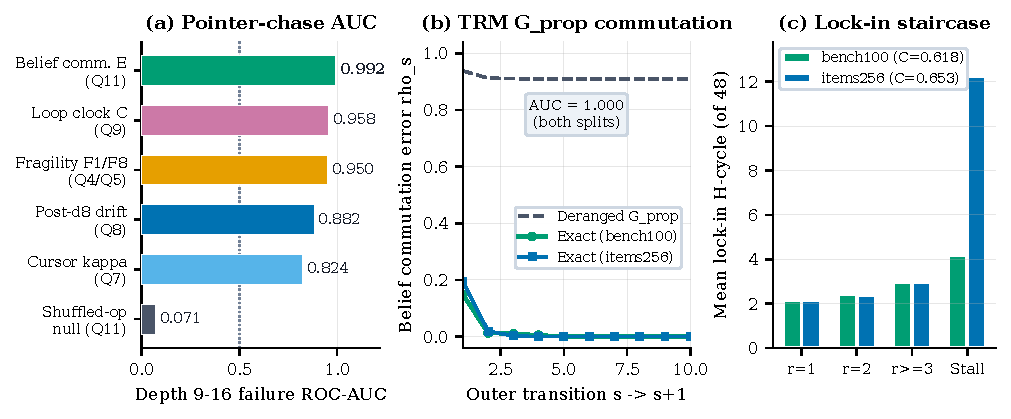
\includegraphics[width=\linewidth]{figures/fig3_compactification_staircase.pdf}
\caption{\textbf{Compactification commutation laws.} \textbf{(a)} ROC-AUC predicting depth-9--16 failure across 24 \texttt{LoopedChase} arms (\texttt{Q11} belief commutation $\hat{E}$ reaches $\mathrm{AUC}=0.992$). \textbf{(b)} Sudoku \texttt{TRM} visible beliefs commute with exact $\Gprop$ ($\rho_{\mathrm{clean}} \to 0.000$ by $s=4$; $\mathrm{AUC}=1.000$ vs.\ deranged clues on both splits). \textbf{(c)} Mean lock-in $H$-cycle (of 48) follows $r=1 < r=2 < r\ge 3 < \text{stalled}$ ($C_{\mathrm{stair}} = 0.653$ vs.\ $0.495$ null on \texttt{items256}).}
\label{fig:compactification}
\end{figure}

\paragraph{The Markovian contrast control for $\Phead$ projection.} To test whether erasing head-orthogonal state harms a Regime II model, we projected the 256-d carried cursor $h_{t,\mathrm{cursor}}$ of all 24 \texttt{LoopedChase} checkpoints onto the 16-d effective row space $\Phead$ of $\texttt{head}\circ\texttt{ln\_f}$ (removing $240/256$ dimensions after every loop $1\dots 16$; Figure~\ref{fig:dark_fiber}b). At $\lambda = 0.1$, \textbf{all $3/3$ seeds retained $1.000$ depth-1--8 and $1.000$ held-out depth-9--16 accuracy} under raw $\Phead$ projection, LayerNorm-moment-preserved projection, donor-swapped orthogonal fiber, and step-1 frozen fiber (and $8/9$ extrapolating $\lambda \in \{0.01, 0.1\}$ seeds across \texttt{Q4}+\texttt{Q5} retained $0.982$--$1.000$). At $\lambda = 1.0$, $2/3$ seeds likewise stayed at $1.000$ while seed 1 dropped to $0.129$ (even with LayerNorm statistics restored, indicating an auxiliary phase coordinate in that single seed; mean $0.710$). Projecting non-cursor edge-table tokens (\texttt{all\_tokens\_fiber\_erased}) collapsed accuracy to $0.177$, as expected because $\texttt{head}$ reads node IDs rather than $(u,v)$ edge bindings. Thus for the carried state variable of a Markovian chain, head-orthogonal cursor dimensions are completely dispensable ($1.000 \to 1.000$ at $\lambda=0.1$).

\section{Regime III: Stationary Attractor Search and Head-Orthogonal Controls}\label{sec:regime3}

We now turn to the frozen 7M-parameter, 2-layer Attention-\texttt{TRM} (\texttt{gaoxin492/\allowbreak TinyRecursiveModels-\allowbreak Sudoku-\allowbreak Extreme-\allowbreak att}, \texttt{step\_21700}, $d=512$, 16 outer steps $\times$ 21 core calls $= 336$ passes; replicated on independent checkpoint \texttt{yagizdevre/\allowbreak trm-\allowbreak sudoku-\allowbreak extreme-\allowbreak att} \cite{jolicoeur2025trm}) across \texttt{items256} ($73$ whole-board $\Gprop$-solvable [\texttt{WB-Prop}], $183$ eventually stalling [\texttt{WB-Stall}]) and \texttt{bench100} ($49$ \texttt{WB-Prop}, $51$ \texttt{WB-Stall}).

\subsection{Two-Timescale Convergence, Corruption Repair, and \texorpdfstring{$\Gprop$}{G\_prop} Commutation (\texttt{P1}--\texttt{P5})}

As audited in Table~\ref{tab:verdicts}, \texttt{TRM} factors Sudoku across two timescales:
\begin{enumerate}[topsep=3pt,itemsep=2pt]
  \item \textbf{Inner 21-call sweep ($s=1$) vs.\ outer steps $s=2\dots 16$:} Step $s=1$ already reaches $0.863$ target-cell accuracy ($1.000$ on \texttt{S1--S2}) but only $0.082$ ($21/256$) exact full-board solve. Outer steps $2\dots 16$ drive exact board solve to $\mathbf{0.883}$ ($226/256$) on \texttt{items256} and $\mathbf{1.000}$ ($100/100$) on \texttt{bench100} ($\mathbf{0.920}$, $92/100$, on the \texttt{yagizdevre} replication checkpoint). Corrupting 10 empty cells of $z_H(1)$ with donor states drops $s=1$ exact board solve to $0.000$ ($0/256$) and self-repairs by $s=16$ to $\mathbf{0.887}$ ($227/256$, $p=9.27\times 10^{-69}$)—exceeding clean $0.883$ ($226/256$) by one board because all $226$ clean-solved boards recover while the step-1 perturbation dislodges one marginally stalled board into the valid basin.
  \item \textbf{Pre-stall $\Gprop$ commutation and post-stall conflict flips:} Visible \texttt{lm\_head} probabilities commute with exact $\Gprop$ on \texttt{WB-Prop} boards ($\rho_s \to 0.000$ by $s=4$, $\mathrm{AUC}=1.000$; Figure~\ref{fig:compactification}b), and lock-in times across all 48 $H$-cycles obey $2.14 < 2.35 < 2.97 < 12.22$ on \texttt{items256} ($C_{\mathrm{stair}}=0.6531$ vs.\ $0.4947$ null; engaging Wu et al.'s \cite{wu2026shared} observation of uneven step progress by tying commit timing directly to deductive round $r(i)$). Past stall, \texttt{TRM} solves $51/51$ ($100\%$) of \texttt{bench100} \texttt{WB-Stall} boards and $153/183$ ($83.6\%$) of \texttt{items256} \texttt{WB-Stall} boards (including $35/64 = 54.7\%$ exact board solve and $48/64 = 75.0\%$ target-cell accuracy on strict round-0 zero-single \texttt{S4\_stalled}), traversing explicit Sudoku unit violations on $98.0\%$--$99.3\%$ of solved stalled boards ($13.90 \to 0.00$ violated units on \texttt{bench100}; Figure~\ref{fig:dark_fiber}a) via $107.8$--$128.0$ non-monotone cell flips.
\end{enumerate}

\begin{table}[t]
\centering
\small
\begin{tabularx}{\linewidth}{@{}ll>{\raggedright\arraybackslash}p{0.31\linewidth}>{\raggedright\arraybackslash}X@{}}
\toprule
Hypothesis & Verdict & Registered threshold behavior & Structural mechanism isolated (with follow-up controls) \\
\midrule
\texttt{P1} Triangulation & Not supported & 3/4 met; single-cell $\Delta_{1\to 16} = +0.074 < 0.25$ & $s{=}1$ (21 core calls) reaches $0.863$ target-cell; $s{=}2..16$ drives full-board exact solve $0.082 \to 0.883$ ($+0.801$) \\
\texttt{P2} Attractor vs.\ VD & Not supported & Repair \& \texttt{NB} drift met; single-cell open drop $0.074 < 0.30$ & 10-cell donor corruption collapses $s{=}1$ board solve to $0.000$ and repairs to $0.887$ ($227/256$); kicks contract $0.303\times$ \\
\texttt{P3} SVD geometry & Weak & \texttt{TRM} $\bar{r}_{\mathrm{outer}}=0.992$, $\bar{r}_{\mathrm{role}}=0.765$; \texttt{NB} $\bar{r}=0.355 \in [0.3, 0.4)$ & \texttt{Nanbeige} SwiGLU multiplexing (\texttt{L12} $0.085$) vs.\ \texttt{TRM} stationary outer operator + inner $z_L/z_H$ role split \\
\texttt{P4} Unrolled \texttt{TCA} & Not supported & Specificity $22.04\% \gg 1.35\%$; $F_1/F_6 = 1{,}808.4 \gg 0.25$ & Detached-ACT tangent expansion (105 calls between $s{=}1,6$ commits) coexists with $0.303\times$ basin contraction \\
\texttt{P5} Compactification & \textbf{Supported} & \textbf{5/5 sub-criteria met} ($p \le 2\times 10^{-28}$) & $\Gprop$ commutation ($\mathrm{AUC}=1.000$); manifold controls split raw $\Phead$ drop into L2-norm loss + stalled-only 64-PCA residual \\
\bottomrule
\end{tabularx}
\caption{Pre-registered \texttt{LOOPSCOPE-02} verdicts and calibrated mechanistic findings.}
\label{tab:verdicts}
\end{table}

\subsection{Dissecting Head-Orthogonal Projection: Off-Manifold Norm Loss vs.\ Stalled-Board Residual}\label{sec:fiber_controls}

Because \texttt{TRM}'s vocabulary has size $11$, $\texttt{lm\_head.weight} \in \mathbb{R}^{11 \times 512}$ has exact rank $11$, defining an 11-d readout row space $\Phead$ and a \textbf{501-dimensional head-orthogonal fiber} $(I - \Phead)\mathbb{R}^{512} = \ker(\texttt{lm\_head})$. In pre-registered test \texttt{P5}, resetting $z_L \leftarrow L_{\mathrm{init}}$ between outer steps preserved $99/100$ ($0.990$) on \texttt{bench100} and $213/256$ ($0.832$) on \texttt{items256}, whereas raw \texttt{fiber\_erased} ($z_H^{\mathrm{board}} \leftarrow z_H^{\mathrm{board}}\Phead + H_{\mathrm{init}}(I-\Phead)$ plus \texttt{reset\_zL}) collapsed solve to $0.070$ ($7/100$ at batch-size 50; $5/100 = 0.050$ under float64 SVD at batch-size 64) on \texttt{bench100}, $0.000$ ($0/100$) on \texttt{yagizdevre} replication, and $0.066$ ($17/256$) on \texttt{items256}.

However, inspecting \texttt{fiber\_erased} \emph{by stratum} exposes a critical confound (Table~\ref{tab:fiber_controls}): raw \texttt{fiber\_erased} (and \texttt{zH\_fiber\_only\_erased}, which keeps $z_L$ live: $0.060$ on \texttt{bench100}, $0.070$ on \texttt{items256}) destroys \textbf{propagation-solvable boards too} ($5/49$ on \texttt{bench100}; $17/73 = 0.233$ on \texttt{items256}, even while single target cells in \texttt{S1}/\texttt{S2} stay at $0.984/0.969$). Why did raw $\Phead$ projection break \texttt{TRM} propagation when it left \texttt{LoopedChase} ($\lambda=0.1$) at $1.000$? In \texttt{LoopedChase}, $h \leftarrow \operatorname{LN}(h) + e$ re-normalizes the projected vector before input addition; in \texttt{TRM}, \texttt{run\_l\_level} feeds $z_H + x_{\mathrm{emb}}$ \emph{without normalization}, so zeroing $501/512$ coordinates collapses $\|z_H\|_2$ against $\sqrt{512}$-scaled $x_{\mathrm{emb}}$ and strips the trained \texttt{Post-RMSNorm} affine carrier offset.

\begin{figure}[t]
\centering
\includegraphics[width=\linewidth]{figures/fig4_dark_fiber_ablation.pdf}
\caption{\textbf{Conflict repair, manifold controls, and head-orthogonal PCA dose-response.} \textbf{(a)} On \texttt{bench100}, \texttt{TRM} solves $49/49$ \texttt{WB-Prop} and $51/51$ \texttt{WB-Stall} boards, driving violated Sudoku units from $13.9 \to 0.0$. \textbf{(b)} Separating off-manifold norm loss from regime-selective fiber dependence: raw $\Phead$ fails on \texttt{TRM Prop} ($0.233$) via unnormalized $\|z_H\|_2$ shrinkage, whereas restoring cell L2 norm or grafting donor fibers preserves $1.000$ on both \texttt{LoopedChase} ($\lambda=0.1$) and \texttt{TRM Prop} ($73/73$), isolating a selective drop on \texttt{WB-Stall} ($0.836 \to 0.749$, $p=8.6\times 10^{-4}$) and \texttt{S4} ($0.547 \to 0.391$; $0.328$ under step-1 freeze). \textbf{(c)} Top-$k$ orthogonal PCA dose curve (fitted strictly on \texttt{train.csv}): $k=64$ ($86.6\%$ variance) recovers full clean solve ($0.831$ vs.\ $0.836$, $p=1.00$).}
\label{fig:dark_fiber}
\end{figure}

\begin{table}[t]
\centering
\scriptsize
\setlength{\tabcolsep}{2.3pt}
\begin{tabular}{@{}lccccccccc@{}}
\toprule
Inter-step condition ($s \ge 1$) & \multicolumn{2}{c}{\texttt{bench100} (Repl.)} & \multicolumn{2}{c}{\texttt{items256} Whole-Board} & \multicolumn{4}{c}{\texttt{items256} Stratum Board [Cell]} & $p_{\mathrm{McNemar}}$ \\
\cmidrule(lr){2-3}\cmidrule(lr){4-5}\cmidrule(lr){6-9}
 & Prop (49) & Stall (51) & Prop (73) & Stall (183) & \texttt{S1} (64) & \texttt{S2} (64) & \texttt{S3} (64) & \texttt{S4} (64) & (\texttt{WB-Stall}) \\
\midrule
Clean $s=16$ (full 512-d) & 1.00 (0.92) & 1.00 (0.92) & \textbf{1.000} & \textbf{0.836} & 1.00 [1.00] & 0.98 [1.00] & 1.00 [1.00] & \textbf{0.55} [0.75] & --- \\
\texttt{reset\_zL} ($z_L \leftarrow L_{\mathrm{init}}$) & 1.00 (0.92) & 0.98 (0.84) & 1.000 & 0.765 & 0.97 [1.00] & 0.95 [1.00] & 0.95 [1.00] & 0.45 [0.72] & $2.4\times 10^{-4}$ \\
Raw \texttt{fiber\_erased} (\texttt{P5}) & 0.10 (0.00) & 0.00 (0.00) & 0.233 & 0.000 & 0.16 [0.98] & 0.02 [0.97] & 0.09 [0.83] & 0.00 [0.50] & $1.8\times 10^{-46}$ \\
\texttt{zH\_fiber\_only\_erased} & 0.12 (0.00) & 0.00 (0.00) & 0.247 & 0.000 & 0.16 [1.00] & 0.06 [0.98] & 0.06 [0.78] & 0.00 [0.56] & $1.8\times 10^{-46}$ \\
\midrule
\texttt{fiber\_norm\_restored} ($k{=}0$) & 1.00 (0.98) & 1.00 (0.88) & \textbf{1.000} & \textbf{0.749} & 0.97 [1.00] & 0.97 [1.00] & 0.95 [1.00] & \textbf{0.39} [0.67] & $8.6\times 10^{-4}$ \\
\texttt{fiber\_train\_mean\_filled} & 1.00 (0.96) & 1.00 (0.96) & \textbf{1.000} & \textbf{0.760} & 0.98 [1.00] & 0.95 [1.00] & 0.97 [1.00] & \textbf{0.41} [0.73] & $4.3\times 10^{-3}$ \\
\texttt{fiber\_donor\_swapped} & 1.00 (0.92) & 1.00 (0.92) & \textbf{1.000} & \textbf{0.754} & 0.97 [1.00] & 0.95 [1.00] & 0.98 [1.00] & \textbf{0.39} [0.69] & $1.5\times 10^{-3}$ \\
\texttt{fiber\_step1\_frozen} & 0.98 (0.98) & 0.92 (0.94) & 0.973 & \textbf{0.678} & 0.94 [1.00] & 0.91 [1.00] & 0.88 [0.98] & \textbf{0.33} [0.66] & $1.1\times 10^{-6}$ \\
\midrule
Orth.\ PCA $k=16$ ($49.9\%$ var) & 1.00 (0.82) & 1.00 (0.90) & 0.986 & 0.798 & 0.97 [1.00] & 0.97 [1.00] & 0.98 [1.00] & 0.48 [0.77] & $0.118$ \\
Orth.\ PCA $k=64$ ($86.6\%$ var) & 1.00 (0.90) & 1.00 (0.78) & \textbf{1.000} & \textbf{0.831} & 1.00 [1.00] & 0.94 [1.00] & 0.98 [1.00] & \textbf{0.59} [0.83] & $1.000$ \\
Orth.\ PCA $k=501$ ($100\%$ var) & 1.00 (0.92) & 1.00 (0.92) & \textbf{1.000} & \textbf{0.836} & 1.00 [1.00] & 0.98 [1.00] & 1.00 [1.00] & \textbf{0.55} [0.75] & $1.000$ \\
\bottomrule
\end{tabular}
\caption{Per-stratum exact 81-cell board solve (with \texttt{yagizdevre} replication in parentheses on \texttt{bench100}, and single target-cell accuracy in brackets on \texttt{items256} \texttt{S1--S4}) across manifold, donor, and train-split orthogonal-fiber PCA controls. Note: on \texttt{WB-Prop} ($n=73$), $p_{\mathrm{McNemar}} = 1.000$ for every manifold-preserving control ($73/73$ solved).}
\label{tab:fiber_controls}
\end{table}

We therefore ran five manifold-preserving and dose-response controls (fitted strictly on $200$ \texttt{train.csv} boards with zero test leakage; Table~\ref{tab:fiber_controls}, Figure~\ref{fig:dark_fiber}b--c), establishing three exact results:
\begin{enumerate}[topsep=3pt,itemsep=2pt]
  \item \textbf{Propagation-solvable boards require zero head-orthogonal information:} Simply rescaling the 11-d projection $z_H^{\mathrm{board}}\Phead$ to each cell's pre-projection L2 norm (\texttt{fiber\_norm\_restored}, carrying \emph{zero} orthogonal dimensions), filling $(I-\Phead)z_H$ with step-$s$ \texttt{train.csv} means (\texttt{fiber\_train\_mean\_filled}), or grafting a \emph{foreign donor board's} live 501-d fiber (\texttt{fiber\_donor\_swapped}) restores \textbf{$49/49$ ($100\%$) on \texttt{bench100} \texttt{WB-Prop} ($45$--$48/49$ on \texttt{yagizdevre}) and $73/73$ ($100\%$, McNemar $p=1.000$) on \texttt{items256} \texttt{WB-Prop}}.
  \item \textbf{Continuous $81\times 11$ logit fields solve most stalled boards, while a 64-PCA head-orthogonal residual supplies $+7.7$ to $+8.7$~pp on hard stalled search:} Because each outer step feeds the entire $81\times 11$ continuous logit field through 21 fresh inner \texttt{L\_level} calls with live $z_L$ and clues $x_{\mathrm{emb}}$, norm-restored 11-d head state alone already solves $51/51$ ($100\%$) of \texttt{bench100} stalled boards ($45/51 = 0.882$ on \texttt{yagizdevre}) and $137/183$ ($74.9\%$) of \texttt{items256} \texttt{WB-Stall} boards. Yet on \texttt{items256} \texttt{WB-Stall}, \emph{every} manifold-preserving erasure leaves a significant, regime-selective deficit relative to clean $153/183$ ($0.836$): \texttt{fiber\_norm\_restored} drops to $137/183$ ($0.749$, $-8.7$~pp, $p=8.55\times 10^{-4}$), \texttt{fiber\_train\_mean\_filled} and \texttt{pca\_k0} to $139/183$ ($0.760$, $-7.7$~pp, $p=0.0043$), \texttt{fiber\_donor\_swapped} to $138/183$ ($0.754$, $-8.2$~pp, $p=0.0015$), and \texttt{fiber\_step1\_frozen} to $124/183$ ($0.678$, $-15.8$~pp, $p=1.08\times 10^{-6}$—worse than neutral mean fill because stale step-1 conflict state misleads later outer steps). On round-0 stalled \texttt{S4\_stalled} ($n=64$), board-exact solve drops from $35/64$ ($0.547$) to $25/64$ ($0.391$, $-15.6$~pp) under norm-restored/donor controls and $21/64$ ($0.328$, $-21.9$~pp) under step-1 freeze. Retaining top-$k$ train-PCA orthogonal directions recovers stalled performance monotonically ($0.760 \to 0.798$ at $k=16 \to \mathbf{0.831}$ [$152/183$, $p=1.000$] at $k=64$, $86.6\%$ variance; \texttt{S4} reaches $38/64 = 0.594$ at $k=64$).
  \item \textbf{Head-orthogonal, not probe-opaque:} Across held-out empty cells, $(I-\Phead)z_H(s)$ leaks $< 1.5\times 10^{-5}$ max absolute logit into \texttt{lm\_head}, yet linear ridge probes trained strictly on \texttt{train.csv} decode from $(I-\Phead)z_H(s)$: (i) initial clue-eliminated candidate masks at $\mathbf{97.7\%}$ (\texttt{bench100}; $98.6\%$ on stalled) and $\mathbf{97.1\%}$ (\texttt{items256}; $97.8\%$ on stalled) at $s=1$, (ii) current step-$s$ \texttt{lm\_head} argmax digits at $97.4\% \to 99.8\% \to 100.0\%$ (\texttt{bench100}) and $95.6\% \to 97.9\% \to 98.8\%$ (\texttt{items256}) across $s \in \{1, 4, 16\}$, and (iii) ground-truth final digits at $80.8\% \to 98.4\% \to 100.0\%$ and $71.2\% \to 88.7\% \to 93.5\%$, matching \texttt{lm\_head}'s own accuracy within $0.2$~pp.
\end{enumerate}

\section{Synthesis: Calibrated Monitorability Boundary and Outlook}\label{sec:discussion}

\paragraph{Two methodological lessons and a calibrated boundary.} Pairing \texttt{HUG-CAL-02} with our \texttt{LOOPSCOPE-02} manifold controls highlights a recurring pitfall in looped-model interpretability: just as uncalibrated SVD ablations conflate late-loop Jacobian fragility with factor specialization, unnormalized subspace projections conflate off-manifold scale collapse with hidden-channel necessity. Once controlled on-manifold:
\begin{itemize}
  \item \textbf{Markovian propagation} (\texttt{LoopedChase} at $\lambda=0.1$, \texttt{WB-Prop} Sudoku) requires \textbf{zero} head-orthogonal state ($1.000$ retention under $\Phead$ norm-restored and donor controls), with $\hat{E}$ predicting extrapolation at $\mathrm{AUC}=0.992$.
  \item \textbf{Post-stall NP search} (\texttt{TRM} on \texttt{WB-Stall} / \texttt{S4} Sudoku) executes $\approx 85\%$--$90\%$ of its successful search directly through the re-injected $81\times 11$ continuous logit field ($74.9\%$ vs.\ $83.6\%$ stalled solve), while relying on a dynamically updated, $\approx 64$-PCA-dimensional \emph{head-orthogonal} ($\ker(\texttt{lm\_head})$) residual for the hardest $8.7$~pp ($15.6$~pp in \texttt{S4}). That residual is invisible to output-logit lenses yet linearly accessible to standard ridge probes ($97.8\%$ candidate-mask accuracy).
\end{itemize}

\paragraph{Limitations and prospective \texttt{ARC-AGI-2} protocol.} Four scope boundaries apply: (i) comparing pretrained \texttt{Nanbeige-3B} and \texttt{Qwen-4B} to puzzle-supervised 7M \texttt{TRM}s separates 3-shot LM inference from detached-ACT puzzle training rather than matched-training recurrence \cite{sesodia2026inside}; (ii) the Detached-ACT vs.\ BPTT Lyapunov contrast is observational without a 336-call BPTT-retrained \texttt{TRM}; (iii) whether continuous JumpReLU dictionaries avoid Top-$k$ support switching in \texttt{Nanbeige} remains open; and (iv) testing universality beyond Sudoku requires running \emph{norm-restored}, \emph{donor-swapped}, and \emph{top-$k$ PCA} $\Phead$ controls on $d=512$, 11-color \texttt{ARC-AGI-2} \texttt{TRM} checkpoints \cite{jolicoeur2025trm} stratified by cellular propagation vs.\ hypothesis revision.

\bibliographystyle{plain}
\bibliography{references}

\end{document}
